%
% The first command in your LaTeX source must be the \documentclass command.
\documentclass[acmlarge,screen]{acmart}

%
% defining the \BibTeX command - from Oren Patashnik's original BibTeX documentation.
\def\BibTeX{{\rm B\kern-.05em{\sc i\kern-.025em b}\kern-.08emT\kern-.1667em\lower.7ex\hbox{E}\kern-.125emX}}
    
% Rights management information. 
% This information is sent to you when you complete the rights form.
% These commands have SAMPLE values in them; it is your responsibility as an author to replace
% the commands and values with those provided to you when you complete the rights form.
%
% These commands are for a PROCEEDINGS abstract or paper.
\copyrightyear{2021}
\acmYear{2021}
% \setcopyright{acmlicensed}
% \acmConference[Woodstock '18]{Woodstock '18: ACM Symposium on Neural Gaze Detection}{June 03--05, 2018}{Woodstock, NY}
% \acmBooktitle{Woodstock '18: ACM Symposium on Neural Gaze Detection, June 03--05, 2018, Woodstock, NY}
% \acmPrice{15.00}
% \acmDOI{10.1145/1122445.1122456}
% \acmISBN{978-1-4503-9999-9/18/06}

%
% These commands are for a JOURNAL article.
%\setcopyright{acmcopyright}
%\acmJournal{TOG}
%\acmYear{2018}\acmVolume{37}\acmNumber{4}\acmArticle{111}\acmMonth{8}
%\acmDOI{10.1145/1122445.1122456}

%
% Submission ID. 
% Use this when submitting an article to a sponsored event. You'll receive a unique submission ID from the organizers
% of the event, and this ID should be used as the parameter to this command.
%\acmSubmissionID{123-A56-BU3}

%
% The majority of ACM publications use numbered citations and references. If you are preparing content for an event
% sponsored by ACM SIGGRAPH, you must use the "author year" style of citations and references. Uncommenting
% the next command will enable that style.
%\citestyle{acmauthoryear}

\DeclareMathOperator*{\argmax}{argmax}

%
% end of the preamble, start of the body of the document source.
\begin{document}

%
% The "title" command has an optional parameter, allowing the author to define a "short title" to be used in page headers.
\title{Deep Reinforcement Learning Algorithms}

%
% The "author" command and its associated commands are used to define the authors and their affiliations.
% Of note is the shared affiliation of the first two authors, and the "authornote" and "authornotemark" commands
% used to denote shared contribution to the research.
\author{Andreas Hofmann}
\email{hofma@csail.mit.edu}

%
% By default, the full list of authors will be used in the page headers. Often, this list is too long, and will overlap
% other information printed in the page headers. This command allows the author to define a more concise list
% of authors' names for this purpose.
\renewcommand{\shortauthors}{Hofmann}

%
% The abstract is a short summary of the work to be presented in the article.
\begin{abstract}
This provides a summary and references for current standard deep reinforcement learning algorithms, including .
\end{abstract}


%
% A "teaser" image appears between the author and affiliation information and the body 
% of the document, and typically spans the page. 
%%\begin{teaserfigure}
%%  \includegraphics[width=\textwidth]{sampleteaser}
%%  \caption{Seattle Mariners at Spring Training, 2010.}
%%  \Description{Enjoying the baseball game from the third-base seats. Ichiro Suzuki preparing to bat.}
%%  \label{fig:teaser}
%%\end{teaserfigure}

%
% This command processes the author and affiliation and title information and builds
% the first part of the formatted document.
% Don't include acm ref.  -agh, 8/12/2021
\settopmatter{printacmref=false}  
\maketitle

\section{Introduction}

\subsection{Algorithm Categorization}

DRL (Deep Reinforcement Learning) Algorithms can be categorized according to a number of characteristics.
These include whether the algorithm 

\begin{itemize}
\item uses a model (\textit{model-based} vs. \textit{model-free});
\item learns a value function or learns a policy directly;
\item is an \textit{on-policy} or \textit{off-policy} algorithm.
\end{itemize}

With model-based RL, a model of state transition (next state given current state
and action) is used.  The model supports searching multiple steps ahead in order to select the optimal action,
based on reward at each step.
This search can be informed by both value and policy heuristics, as was done in Alpha Go [cite].
With model-free RL, no explicit state transition model is used.
Instead, one or both of two simpler functions (value function and/or policy function) is learned directly.

A value function returns a scalar value for a given current state.  Related to this, a Q function (or value-action function)
returns a scalar value given a current state and a proposed action from this state.  
These scalar values represent the discounted reward, or future utility, that is expected to accrue, if a particular control
policy is followed.  The Q function can be used to pick the best action given a current state (the action that maximizes reward).
A policy function directly returns an action for a given current state.
Ideally, the policy function is learned well enough that it closely approximates the \textit{optimal} policy function
(returns the best action for a given current state).

An \textit{actor-critic} approach uses both value and policy functions.

In order to understand the difference between on-policy and off-policy methods, it is important to consider and separate out
the policy being learned and the policy used to generate the data.
For on-policy methods, these are the same.
For off-policy methods, these are not the same.
For example, in Q-learning (value function and Q function learning), the policy used to control the agent in the environment
(to generate the data) is only sometimes the policy being learned.  
In particular, the action is sometimes chosen from the policy being learned (greedy option), and is sometimes chosen randomly
(exploratory option).  
This helps to ensure that the learning does not prematurely converge to a local optimum that is significantly less optimal
than the global optimum.
Selection of whether to choose the greedy or exploratory action is based on an \textit{epsilon} factor that decays over time, 
so that as the policy is learned, selection of the greedy action becomes more likely
(leveraging the fact that the policy should be getting better over time).

Q-Learning is an example of an off-policy method.
SARSA is an example of an on-policy method.
See also \url{https://analyticsindiamag.com/reinforcement-learning-policy}.


\noindent See also 
\url{https://smartlabai.medium.com/reinforcement-learning-algorithms-an-intuitive-overview-904e2dff5bbc}

\url{https://www.guru99.com/reinforcement-learning-tutorial.html}

\url{https://en.wikipedia.org/wiki/Deep_reinforcement_learning#Off-policy_reinforcement_learning}

\url{https://analyticsindiamag.com/reinforcement-learning-policy}.


Additional characteristics used to categorize DRL algorithms include:

\begin{itemize}
\item whether the output action is discrete or continuous;
\item whether the input is raw pixels or a state estimate vector;
\item whether the system is deterministic or stochastic.
\end{itemize} 

[Investigate whether there are algorithms that have hybrid discrete/continuous output actions.]

In principle, DRL algorithms model Markov Decision Processes (MDPs).
As such, they are based on the notion of state.
However, in many cases, the distinction between state and sensor data is blurred.
For example, in many DRL algorithms, an environment like the cart-pole environment in the Open AI gym 
provides pixels as the state, rather than the traditional position and angle state estimate, even
though, from a traditional control systems standpoint, pixels should be regarded as sensor input.
This blurring can be considered a feature as it allows for end to end control algorithms.

Regarding whether the system is deterministic or stochastic, a general MDP supports a stochastic environment,
where a particular control action given a current state implies a distribution of possible next states.
The deterministic case is just the degenerate case of the MDP, where the control action implies a single next state.
There is some confusion about this terminology in some of the DRL algorithms;  in some cases, stochastic
implies a control policy that provides a distribution of possible actions given the current state.
Thus, it is possible to have both a distribution of possible actions, and a distribution of next states
conditioned for each action.



\subsection{Algorithm Summaries}


Intro to algorithms (summary of each)
List algorithms, organized (see web sites)






deterministic vs. stochastic, MDP

Confusion about this also






\subsection{To Do}

Focus on continuous action models like mountain car.

Think about whether it makes sense to have hybrid discrete/continuous actions, maybe
from two separate heads of the DNN.



\section{DQN}

Q value algorithm


\subsection{Agent, Reward, Value Function, Q Function, and Policy}

In Reinforcement Learning, an \textit{agent} takes actions in an environment in order to accumulate \textit{rewards}.
The immediate reward at time increment $t$ is given as $R_t$.
When learning how an agent should behave, it is useful to consider \textit{cumulative} reward, 
rather than just immediate reward.
Cumulative reward is defined as the total reward accumulated by the agent over some time horizon:

\begin{equation}
  C_t = R_t + R_{t+1} + R_{t+2} + \ldots = \sum_{k=0}^T R_{t+k} 
\end{equation}

Here, the agent takes actions at regular time increments, denoted by $k$.  
The time horizon, $T$, is specified in terms of the maximum value for $k$.

In practice, when learning agent behaviors, it is useful to favor immediate reward over future reward. 
This is expressed as \textit{discounted} reward, using a discount rate, $\gamma$:
  
\begin{equation}
  G_t = R_t + \gamma R_{t+1} + \gamma^2 R_{t+2} + \ldots = \sum_{k=0}^T \gamma^k R_{t+k} 
\end{equation}

With the discount rate, $T$ is usually set at infinity

\begin{equation}
  G_t = \sum_{k=0}^\infty \gamma^k R_{t+k} 
\end{equation}

The discount rate implies a time horizon in that rewards diminish significantly in the distant future.

A policy, $\pi$, specifies an action, $a$, to be taken by the agent when the state is $s$.  
Two important functions can be defined with respect to a policy.
First, a value function gives the total expected reward given a current state, $s_t$, 
if a particular policy, $\pi$, is followed.

\begin{equation}
  v_\pi (s) = \mathbb{E} \left( G_t \vert S_t = s \right)
\end{equation}

Second, an action-value or \textit{Q} function gives the total expected reward given a current state, $s_t$, 
a current action, $A_t$,
and a particular policy, $\pi$, to be followed (for future actions).

\begin{equation}
  q_\pi (s,a) = \mathbb{E} \left( G_t \vert S_t = s, A_t = a \right)
\end{equation}

The policy can be expressed in terms of the Q function as

\begin{equation}
  \pi(s) = \argmax_a q_\pi (s,a)
\end{equation}

Note that this is circular;  the Q function is, itself, a function of the policy.  
Thus, the challenge is how to compute (learn) the Q function.
To accomplish this, we leverage the Bellman equation:

\begin{equation} \label{eq:tempdiff1}
  q_\pi (s,a) = r + \gamma q_\pi (s^\prime, \pi(s^\prime)) = r + \gamma \argmax_{a^\prime} q_\pi (s^\prime, a^\prime)
\end{equation}

\noindent where $r$ is the immediate reward for action $a$, $s^\prime$ is the next state resulting from taking
action $a$ at state $s$, and $a^\prime$ is the action to be taken at state $s^\prime$.



\subsection{Training: Loss Function, Agent Steps, Replay Memory, and Policy Update}


The \textit{temporal difference error}, $\delta$, is defined as the difference between the two sides of \ref{eq:tempdiff1}:

\begin{equation} \label{eq:tempdiff1}
 \delta =  q_\pi (s,a) = - \left( r + \gamma \argmax_{a^\prime} q_\pi (s^\prime, a^\prime) \right)
\end{equation}

During training, RL algorithms strive to update $q_\pi (s,a)$ so that $\delta$ approaches 0.
In (non-deep) RL, $q_\pi (s,a)$ is represented as a table, and is updated by:

\begin{equation} \label{eq:qupdate}
 q_\pi (s,a) = q_\pi (s,a) + \alpha \left( r + \gamma \argmax_{a^\prime} q_\pi (s^\prime, a^\prime) - q_\pi (s,a) \right)
\end{equation}

\noindent where $\alpha$ is the learning rate.

In Deep Reinforcement Learning, $q_\pi (s,a)$ is represented using a Deep Neural Net rather than a table.
Training (minimization of $\delta$) is accomplished by defining a loss based on $\delta$.
In the PyTorch DQN tutorial (\url{https://pytorch.org/tutorials/intermediate/reinforcement\_q\_learning.html}),
a \textit{Huber Loss} function is used.
This loss, $\mathcal{L}$, is defined as 


\begin{equation}  \label{eq:huberloss}
  \mathcal{L} =
    \begin{cases}
      \frac{1}{2} \delta^2 & \text{for $\lvert \delta \rvert \leq 1$,}\\
      \lvert \delta \rvert - \frac{1}{2} & \text{otherwise.}
    \end{cases}       
\end{equation}

Training occurs over some specified number of episodes (50, for example).
Within each episode, the environment state is first re-initialized, and then the agent explores the environment by taking
\textit{steps}.
For each step, the agent takes an action, resulting in a reward, and a transition from the current state to the next state.
Thus, a step can be summarized by the tuple $\left< \text{state action next-state reward} \right>$.
An episode ends when the environment decides this (usually because the agent has entered a failure state), 
or at some specified limit on the number of steps per episode.

After each step, the result tuple is entered into \textit{replay memory}.  
Replay memory is a buffer of these tuples with a limited size (10000 for example).
As result tuples are added to the end of replay memory, old results are dropped from the beginning.
Thus, replay memory stores the last n (10000 for example) results of experiment steps taken by the agent.

After each agent step, the Q model is updated (optimized).
This is accomplished not by using the results from the most recent step, but rather, by sampling a \textit{batch}
of results from replay memory. 
A typical batch size is 128.
Leveraging the Huber loss function defined above, the loss for the entire batch is defined as

\begin{equation}  \label{eq:batchloss}
  \mathcal{L}_B = \frac{1}{\lvert B \rvert} \sum_{ \left( s,a,s^\prime , r \right) \in B}  \mathcal{L}
\end{equation}

\noindent Model weights are then updated using standard back propagation, based on this loss for the batch.

Experience replay memory ensures that the experience samples in a batch are not correlated;
that they are not overly biased towards results from the most recent policy (model weights).
This stabilizes and improves DQN training.

As in traditional reinforcement learning, the action selected by an agent during a step is sometimes 
\textit{greedy} (following the current learned policy), and is sometimes \textit{exploratory} (random).
The probability of selecting a random action starts high (at 0.9, for example), and then decays exponentially to
a small value (0.05, for example).



\subsection{Policy and Target Networks}

During training, two parallel networks are used:  \textit{policy} network, and \textit{target} network.  
The policy network weights are updated at each training step, using standard back propagation.
The target network weights are kept fixed for most steps;  they are updated at a specified interval
(every 10 training steps for example) from the policy network weights.
The policy network is used to compute the left side of \ref{eq:tempdiff1}.  
The target network is used to compute $q_\pi (s^\prime, a^\prime)$ for the right side of \ref{eq:tempdiff1}.  
Using a separate target network in this way improves training stability.



\subsection{Template Styles}


\begin{verbatim}
  \documentclass[STYLE]{acmart}
\end{verbatim}

Journals use one of three template styles. All but three ACM journals use the {\verb|acmsmall|} template style:
\begin{itemize}
\item {\verb|acmsmall|}: The default journal template style.
\item {\verb|acmlarge|}: Used by JOCCH and TAP.
\item {\verb|acmtog|}: Used by TOG.
\end{itemize}


\section{Tables}

The ``\verb|acmart|'' document class includes the ``\verb|booktabs|'' package --- \url{https://ctan.org/pkg/booktabs} --- for preparing high-quality tables. 

Table captions are placed {\it above} the table.

Because tables cannot be split across pages, the best placement for them is typically the top of the page nearest their initial cite.  To ensure this proper ``floating'' placement of tables, use the environment \textbf{table} to enclose the table's contents and the table caption.  The contents of the table itself must go in the \textbf{tabular} environment, to be aligned properly in rows and columns, with the desired horizontal and vertical rules.  Again, detailed instructions on \textbf{tabular} material are found in the \textit{\LaTeX\ User's Guide}.

Immediately following this sentence is the point at which Table~\ref{tab:freq} is included in the input file; compare the placement of the table here with the table in the printed output of this document.

\begin{table}
  \caption{Frequency of Special Characters}
  \label{tab:freq}
  \begin{tabular}{ccl}
    \toprule
    Non-English or Math&Frequency&Comments\\
    \midrule
    \O & 1 in 1,000& For Swedish names\\
    $\pi$ & 1 in 5& Common in math\\
    \$ & 4 in 5 & Used in business\\
    $\Psi^2_1$ & 1 in 40,000& Unexplained usage\\
  \bottomrule
\end{tabular}
\end{table}

To set a wider table, which takes up the whole width of the page's live area, use the environment \textbf{table*} to enclose the table's contents and the table caption.  As with a single-column table, this wide table will ``float'' to a location deemed more desirable. Immediately following this sentence is the point at which Table~\ref{tab:commands} is included in the input file; again, it is instructive to compare the placement of the table here with the table in the printed output of this document.

\begin{table*}
  \caption{Some Typical Commands}
  \label{tab:commands}
  \begin{tabular}{ccl}
    \toprule
    Command &A Number & Comments\\
    \midrule
    \texttt{{\char'134}author} & 100& Author \\
    \texttt{{\char'134}table}& 300 & For tables\\
    \texttt{{\char'134}table*}& 400& For wider tables\\
    \bottomrule
  \end{tabular}
\end{table*}

\section{Math Equations}
You may want to display math equations in three distinct styles:
inline, numbered or non-numbered display.  Each of
the three are discussed in the next sections.

\subsection{Inline (In-text) Equations}
A formula that appears in the running text is called an
inline or in-text formula.  It is produced by the
\textbf{math} environment, which can be
invoked with the usual \texttt{{\char'134}begin\,\ldots{\char'134}end}
construction or with the short form \texttt{\$\,\ldots\$}. You
can use any of the symbols and structures,
from $\alpha$ to $\omega$, available in
\LaTeX~\cite{Lamport:LaTeX}; this section will simply show a
few examples of in-text equations in context. Notice how
this equation:
\begin{math}
  \lim_{n\rightarrow \infty}x=0
\end{math},
set here in in-line math style, looks slightly different when
set in display style.  (See next section).

\subsection{Display Equations}
A numbered display equation---one set off by vertical space from the
text and centered horizontally---is produced by the \textbf{equation}
environment. An unnumbered display equation is produced by the
\textbf{displaymath} environment.

Again, in either environment, you can use any of the symbols
and structures available in \LaTeX\@; this section will just
give a couple of examples of display equations in context.
First, consider the equation, shown as an inline equation above:
\begin{equation}
  \lim_{n\rightarrow \infty}x=0
\end{equation}
Notice how it is formatted somewhat differently in
the \textbf{displaymath}
environment.  Now, we'll enter an unnumbered equation:
\begin{displaymath}
  \sum_{i=0}^{\infty} x + 1
\end{displaymath}
and follow it with another numbered equation:
\begin{equation}
  \sum_{i=0}^{\infty}x_i=\int_{0}^{\pi+2} f
\end{equation}
just to demonstrate \LaTeX's able handling of numbering.

\section{Figures}

The ``\verb|figure|'' environment should be used for figures. One or more images can be placed within a figure. If your figure contains third-party material, you must clearly identify it as such, as shown in the example below.
\begin{figure}[h]
  \centering
  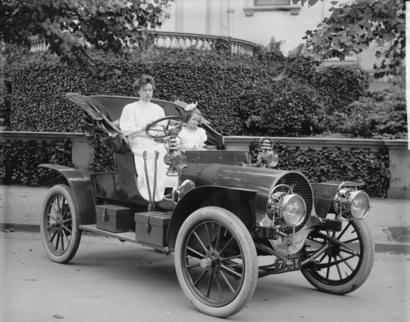
\includegraphics[width=\linewidth]{sample-franklin}
  \caption{1907 Franklin Model D roadster. Photograph by Harris \& Ewing, Inc. [Public domain], via Wikimedia Commons. (\url{https://goo.gl/VLCRBB}).}
  \Description{The 1907 Franklin Model D roadster.}
\end{figure}

Your figures should contain a caption which describes the figure to the reader. Figure captions go below the figure. Your figures should {\bf also} include a description suitable for screen readers, to assist the visually-challenged to better understand your work.

Figure captions are placed {\it below} the figure.


\section{Citations and Bibliographies}

The use of \BibTeX\ for the preparation and formatting of one's references is strongly recommended. Authors' names should be complete --- use full first names (``Donald E. Knuth'') not initials (``D. E. Knuth'') --- and the salient identifying features of a reference should be included: title, year, volume, number, pages, article DOI, etc. 

The bibliography is included in your source document with these two commands, placed just before the \verb|\end{document}| command:
\begin{verbatim}
  \bibliographystyle{ACM-Reference-Format}
  \bibliography{bibfile}
\end{verbatim}
where ``\verb|bibfile|'' is the name, without the ``\verb|.bib|'' suffix, of the \BibTeX\ file.

Citations and references are numbered by default. A small number of ACM publications have citations and references formatted in the ``author year'' style; for these exceptions, please include this command in the {\bf preamble} (before ``\verb|\begin{document}|'') of your \LaTeX\ source: 
\begin{verbatim}
  \citestyle{acmauthoryear}
\end{verbatim}

Some examples.  A paginated journal article \cite{Abril07}, an enumerated journal article \cite{Cohen07}, a reference to an entire issue \cite{JCohen96}, a monograph (whole book) \cite{Kosiur01}, a monograph/whole book in a series (see 2a in spec. document)
\cite{Harel79}, a divisible-book such as an anthology or compilation \cite{Editor00} followed by the same example, however we only output the series if the volume number is given \cite{Editor00a} (so Editor00a's series should NOT be present since it has no vol. no.),
a chapter in a divisible book \cite{Spector90}, a chapter in a divisible book in a series \cite{Douglass98}, a multi-volume work as book \cite{Knuth97}, an article in a proceedings (of a conference, symposium, workshop for example) (paginated proceedings article) \cite{Andler79}, a proceedings article with all possible elements \cite{Smith10}, an example of an enumerated proceedings article \cite{VanGundy07}, an informally published work \cite{Harel78}, a doctoral dissertation \cite{Clarkson85}, a master's thesis: \cite{anisi03}, an online document / world wide web resource \cite{Thornburg01, Ablamowicz07, Poker06}, a video game (Case 1) \cite{Obama08} and (Case 2) \cite{Novak03} and \cite{Lee05} and (Case 3) a patent \cite{JoeScientist001}, work accepted for publication \cite{rous08}, 'YYYYb'-test for prolific author \cite{SaeediMEJ10} and \cite{SaeediJETC10}. Other cites might contain 'duplicate' DOI and URLs (some SIAM articles) \cite{Kirschmer:2010:AEI:1958016.1958018}. Boris / Barbara Beeton: multi-volume works as books \cite{MR781536} and \cite{MR781537}. A couple of citations with DOIs: \cite{2004:ITE:1009386.1010128,Kirschmer:2010:AEI:1958016.1958018}. Online citations: \cite{TUGInstmem, Thornburg01, CTANacmart}.



\section{SIGCHI Extended Abstracts}

The ``\verb|sigchi-a|'' template style (available only in \LaTeX\ and not in Word) produces a landscape-orientation formatted article, with a wide left margin. Three environments are available for use with the ``\verb|sigchi-a|'' template style, and produce formatted output in the margin:
\begin{itemize}
\item {\verb|sidebar|}:  Place formatted text in the margin.
\item {\verb|marginfigure|}: Place a figure in the margin.
\item {\verb|margintable|}: Place a table in the margin.
\end{itemize}

%
% The acknowledgments section is defined using the "acks" environment (and NOT an unnumbered section). This ensures
% the proper identification of the section in the article metadata, and the consistent spelling of the heading.
\begin{acks}
To Robert, for the bagels and explaining CMYK and color spaces.
\end{acks}

%
% The next two lines define the bibliography style to be used, and the bibliography file.
\bibliographystyle{ACM-Reference-Format}
\bibliography{sample-base}

% 
% If your work has an appendix, this is the place to put it.
\appendix

\section{Useful web references}


\subsection{Introduction to Deep Learning}

% Sutton and Barto
\noindent \url{http://incompleteideas.net/book/the-book.html}

\noindent \url{https://markus-x-buchholz.medium.com/deep-reinforcement-learning-introduction-deep-q-network-dqn-algorithm-fb74bf4d6862}

\noindent \url{https://www.kdnuggets.com/2018/03/5-things-reinforcement-learning.html}

\noindent \url{https://www.guru99.com/reinforcement-learning-tutorial.html}

\noindent \url{https://deepmind.com/blog/article/deep-reinforcement-learning}

\noindent \url{https://smartlabai.medium.com/reinforcement-learning-algorithms-an-intuitive-overview-904e2dff5bbc}

\noindent \url{https://en.wikipedia.org/wiki/Deep_reinforcement_learning#Off-policy_reinforcement_learning}


\subsection{DQN}

\noindent \url{https://pytorch.org/tutorials/intermediate/reinforcement\_q\_learning.html}

\noindent \url{https://unnatsingh.medium.com/deep-q-network-with-pytorch-d1ca6f40bfda}

\noindent \url{https://www.toptal.com/deep-learning/pytorch-reinforcement-learning-tutorial}

\noindent \url{https://towardsdatascience.com/deep-q-learning-tutorial-mindqn-2a4c855abffc}

\noindent \url{https://towardsdatascience.com/dqn-part-1-vanilla-deep-q-networks-6eb4a00febfb}

\noindent \url{https://en.wikipedia.org/wiki/Q-learning}

\noindent \url{https://openai.com/blog/openai-baselines-dqn/}


\subsection{General Algorithms and Repositories}

\noindent \url{https://github.com/p-christ/Deep-Reinforcement-Learning-Algorithms-with-PyTorch}

\noindent \url{https://github.com/openai/baselines}


\subsection{Reference Papers and Surveys}

\noindent \url{https://spinningup.openai.com/en/latest/spinningup/keypapers.html}

\noindent \url{https://arxiv.org/abs/1906.10025}



\subsection{Latex}

\noindent \url{https://www.latextemplates.com/template/acm-publications}

\noindent \url{http://math.mit.edu/~dspivak/files/symbols-all.pdf}


\end{document}
